\documentclass{article}
\usepackage{graphicx}
\usepackage[hidelinks]{hyperref}
\usepackage{titlesec}
\usepackage{fancyvrb}
\usepackage{subcaption}
\captionsetup{compatibility=false}
\graphicspath{ {./images/} }
\titleformat{\chapter}{}{}{0em}{\bf\LARGE}
\titlespacing*{\chapter}{0pt}{40pt}{10pt}

\usepackage{geometry}
 \geometry{
 a4paper,
 total={170mm,257mm},
 left=20mm,
 top=20mm,
 }

\usepackage{etoolbox}
\makeatletter
\patchcmd{\chapter}{\if@openright\cleardoublepage\else\clearpage\fi}{}{}{}
\makeatother

\title{
\includegraphics[width=8cm]{bashlogo.png} \\[2cm] CS 108 - Bash Grader}
\author{Siddhant Mulkikar}
\date{\today}

\begin{document}

\maketitle
\newpage
\tableofcontents
\newpage

\section{Objective}
The objective of this CS108 Project was to create a csv file manager and interpreter with a command line interface.

\section{Introduction}
Bash Grader is a command line interface for instructors to grade students and manage their marks. It is an incredibly useful tool with its many functionalities and features. 

\section{List of Functionalities}
\subsection{Basic functionalities}
\begin{itemize}
    \item Upload a marklist in the form of a csv file.
    \item Total the marks of each student over all exams
    \item Combine the marks of all exams into a single csv file
    \item Update the marks of a student in a particular exam or add a student's record to an exam
    \item Implement a working git system with init, add, commit and checkout functionalities
\end{itemize}
\subsection{Customisations}
\begin{itemize}
    \item A staging area with add and remove funtionalities.
    \item A diff patch system for the checkout functionality
    \item Commit history log
    \item Graphs for a particular exam or all exams
    \item Stats for a particular exam or all exams
    \item Report card generation for all students with grade calculation for all students, based on manual rubrics from the instructor/user
    \item Ranked marklists for a particular exam or all exams
    \item Shows git head
\end{itemize}
\newpage
\section{Usage}
\subsection{Upload}
Run the following command to upload a csv file in your current directory.
\begin{verbatim}
    bash submission.sh upload <filename>
\end{verbatim}


\subsection{Total}
Run the following command to total the marks of each student over all exams into a total column in \verb"main.csv".
\begin{Verbatim}
    bash submission.sh total
\end{Verbatim}


\subsection{Combine}
The following command combines all the csv files in the current directory into \verb"main.csv".
\begin{Verbatim}
    bash submission.sh combine
\end{Verbatim}


\subsection{Update}
Run the following command to update the marks of a particular student or add a student's record to an exam.
\begin{verbatim}
    bash submission.sh update
\end{verbatim}

\subsection{Rank}
Run the following command to get the ranked marklist for a particular exam or \verb"main.csv".
\begin{verbatim}
    bash submission.sh rank <exam-name>
\end{verbatim}

\subsection{Git Init}
Run the following command to initialize a remote git repository.
\begin{verbatim}
    bash submission.sh git_init <remote-repo-path>
\end{verbatim}

\subsection{Git Add}
Run the following command to add files from the current directory to the staging area.
\begin{verbatim}
    bash submission.sh git_add
\end{verbatim}

\subsection{Git Remove}
Run the following command to remove files from the staging area.
\begin{verbatim}
    bash submission.sh git_remove
\end{verbatim}

\subsection{Git Commit}
Run the following command to commit the files in the staging area to the remote repository.
\begin{verbatim}
    bash submission.sh git_commit -m "commit message"
\end{verbatim}

\subsection{Git Checkout}
Run the following command to checkout a particular commit from the remote repository.
\begin{verbatim}
    bash submission.sh git_checkout <commit-id> 
    bash submission.sh git_checkout -m <commit-message>
\end{verbatim}
\newpage

\subsection{Git Log}
Run the following command to get the commit history log.
\begin{verbatim}
    bash submission.sh git_log
\end{verbatim}

\subsection{Git Head}
Run the following command to get the head of the git repository, i.e. the current version of directory.
\begin{verbatim}
    bash submission.sh git_head
\end{verbatim}

\subsection{Graphs}
Run the following command to get the graphs for a particular exam or all exams.
\begin{verbatim}
    bash submission.sh graphs
\end{verbatim}

\subsection{Stats}
Run the following command to get the stats for a particular exam or \verb"main.csv".
\begin{verbatim}
    bash submission.sh stats
\end{verbatim}

\subsection{Report Card}
Run the following command to get the report card/s for a particular student or all students.  
\begin{verbatim}
    bash submission.sh report_card
\end{verbatim}

\section{Working}
\subsection{Upload}
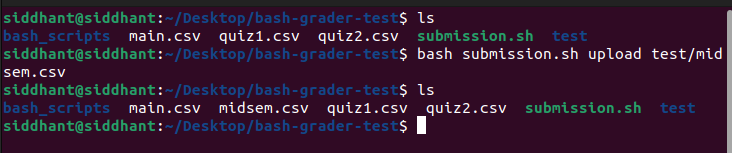
\includegraphics[width=\textwidth]{upload.png}
In the above example, the file \verb"quiz1.csv" is uploaded i.e. copied into the current directory from the filepath given as argument by the user.
The script checks if the file exists and if it is a csv file. If it is, only then is the file copied into the current directory.\\
\textbf{Script files : upload.sh }


\subsection{Total}
\begin{center}
    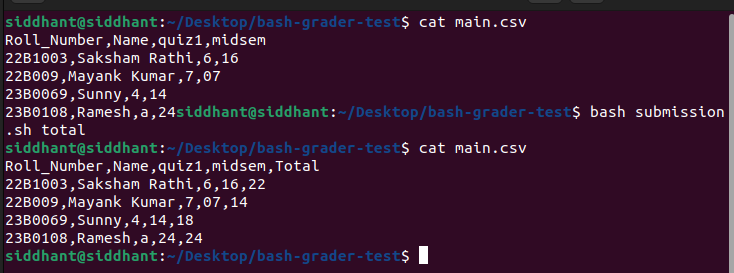
\includegraphics[width=10cm]{total.png}
\end{center}
In the above example, the script totals the marks of each student over all exams and adds a new column \verb"Total" to the \verb"main.csv" file.
If the marks column has \verb"a" as its entry, the script skips that row while totaling.\\
\textbf{Script files : total.awk }

\subsection{Combine}
In the below example, the script combines all the csv files in the current directory into a single \verb"main.csv" file. The script checks if the file is a csv file and if it is not the \verb"main.csv" file.\\ \verb"main.csv" is constructed from scratch in the following steps:
\begin{enumerate}
    \item First, an array of all unique roll numbers and names is created.
    \item Then, based on the exam files, a header is created with the roll numbers and names.
    \item A mesh of \verb"a"'s is created with the dimensions of the header.
    \item Then the script iterates over all exam files and fills in the marks of each student in the mesh, whenever they are found. This ensures that anyone who is not present in a particular exam file is marked as \verb"a"(absent) in \verb"main.csv" for that particular exam.
\end{enumerate}
\begin{figure}[h]
    \begin{subfigure}{0.5\textwidth}
    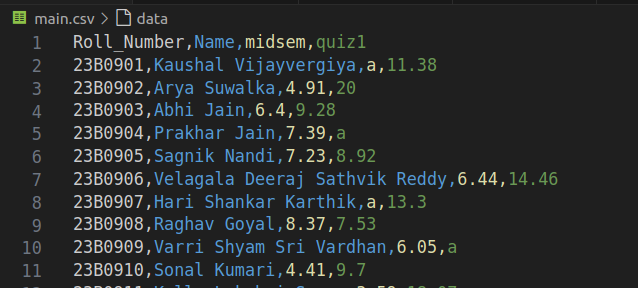
\includegraphics[width=\linewidth, height=3cm]{before_combine.png} 
    \caption{Before combine}
    \label{fig:subim1}
    \end{subfigure}
    \begin{subfigure}{0.5\textwidth}
    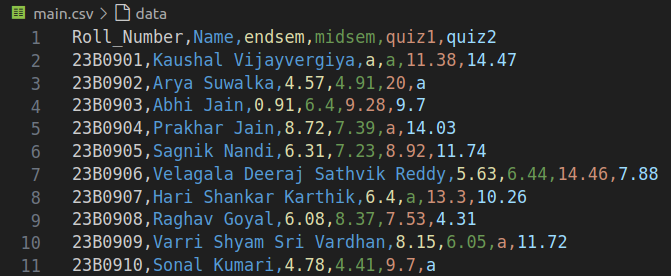
\includegraphics[width=\linewidth, height=3cm]{after_combine.png}
    \caption{After combine}
    \label{fig:subim2}
    \end{subfigure}
\end{figure}

\textbf{Script files : combine.sh, combine.awk}


\subsection{Update}
\begin{figure}[h]
    \begin{subfigure}{0.5\textwidth}
    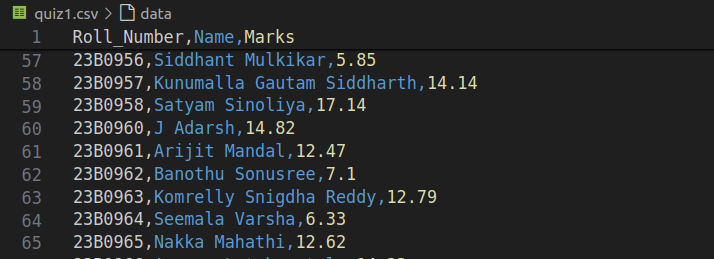
\includegraphics[width=\linewidth, height=3cm]{quiz-before.png} 
    \caption{quiz1.csv before update}
    \end{subfigure}
    \begin{subfigure}{0.5\textwidth}
    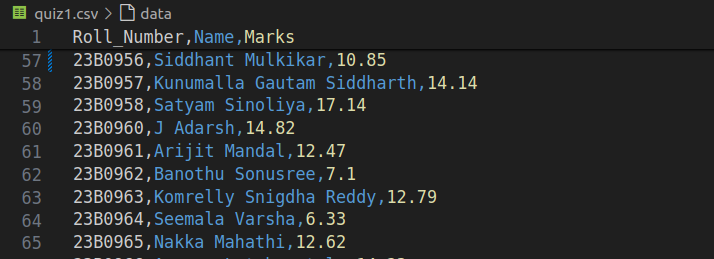
\includegraphics[width=\linewidth, height=3cm]{quiz-after.png}
    \caption{quiz2.csv after update}
    \end{subfigure}
\end{figure}
\begin{figure}[h]
    \begin{subfigure}{0.5\textwidth}
    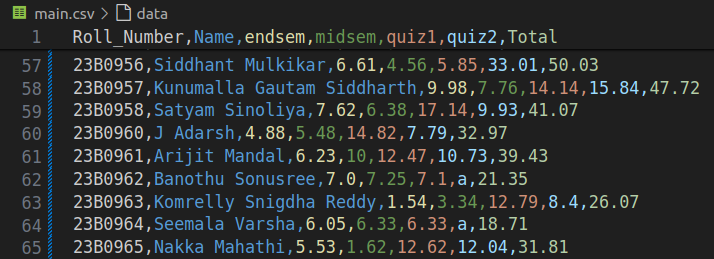
\includegraphics[width=\linewidth, height=3cm]{main-before.png} 
    \caption{main.csv before update}
    \end{subfigure}
    \begin{subfigure}{0.5\textwidth}
    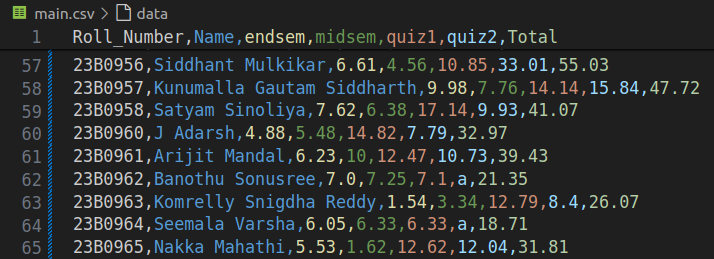
\includegraphics[width=\linewidth, height=3cm]{main-after.png}
    \caption{main.csv after update}
    \end{subfigure}
\end{figure}
In the above example, the script updates the marks of \textbf{23B0956} in \verb"quiz1.csv" and \verb"main.csv".\\
The script first asks the user for the roll number and name of the student whose marks are to be updated. It then checks if the student's name matches with the name paired up with the roll number given by the user. If the names do not match, the script confirms with the user with a prompt for the correct name.\\
It then checks if the student is present in the \verb"main.csv" file and if the exam file exists. If the student is present in the \verb"main.csv" file, the script updates the marks of the student in \verb"main.csv" by calling \verb"update_main.awk" and the exam file by calling \verb"update_exam.awk".\\
If the student's record does not exist in the \verb"main.csv" file, the script prompts the user to confirm if they want to add the student's record to an exam file and \verb"main.csv". If the user confirms, the script adds the student's record to the exam file and \verb"main.csv".\\
It also asks the user if they want to update the marks of the student in some other exam and repeats the same process. If the user does not want to update the marks of the student in any other exam, the script checks if \verb"main.csv" had been totaled before. If it was, then the script calls \verb"total.awk" to correct the total, as the marks in \verb"main.csv" have been updated.\\

\textbf{Script files : update.sh, update\_exam.awk, update\_main.awk, total.awk} 

\subsection{Rank}
This commands takes the examname as a command line argument and ranks the students based on the marks in that exam.
If the user enters \verb"main" as the examname, the script ranks the students based on the total marks in \verb"main.csv". The ranked marklists are sorted according to rank and are stored in the folder \verb"ranked_marklists" in the current directory.\\

\textbf{Script files : rank.sh }

\subsection{Git Init}
This command initializes a remote git repository at the path given by the user as a command line argument.\\
It also checks if the path given is a valid path. If a remote repository is already initialized for the current directory, the script prompts the user to confirm if they want to reinitialize the repository.
If the user confirms, the script reinitializes a fresh remote repository at the path provided by the user.\\ 

It also creates a hidden folder \verb".gitrepo" in the current directory. This folder contains a hidden file \verb".gitreponame" which stores the name of the remote repository and \verb".git_log" which records the commit history.\\

Apart from initialization, the script also copies all the csv files in the current directory at the time of initialization to a hidden folder \verb".ogfiles" in the remote repository. The \verb".ogfiles" folder contains the first version of every file which was ever committed. This serves as a refernce point for all files, for my \textbf{diff patch} system for \verb"git\_checkout" to work.\\

\textbf{Script files : git\_init.sh}
\subsection{Git Add}
This command first checks if a remote repository has been initialized for the current directory. If it has not, the script prompts the user to initialize a remote repository first.\\
This command then prompts the user to enter all the files, which they want to add to the staging area, separated by spaces. It then copies all the files to the staging area in the remote repository. If any particular file doesnt exist in the current directory, it gives an error message.\\
\textbf{Script files : git\_add.sh}

\subsection{Git Remove}
This command first checks if a remote repository has been initialized for the current directory. If it has not, the script prompts the user to initialize a remote repository first.\\
It then prompts the user to enter all the files, which they want to remove from the staging area, separated by spaces. It then deletes all the files from the staging area in the remote repository. If any particular file doesnt exist in the staging area, it gives an error message.\\

\textbf{Script files : git\_remove.sh}

\subsection{Git Commit}
The command first checks if a remote repository has been initialized for the current directory. If it has not, the script prompts the user to initialize a remote repository first.\\
It then checks what all files in the staging area are modified with respect to the first version of the file in the \verb".ogfiles" folder. It also checks for any new files which were created and committed for the first time. It then updates the \verb".git_log" file with these modified and added files, along with the commit message and the files which were modified or added in this commit, which is uniqely identified by the commit message, given by the user and the 16 character hash commit id, generated randomly using the \verb"uuidgen" command. A folder with the commit-id as its name is created in the commits folder of the remote repository.\\

If any file in the staging area is not present in the \verb".ogfiles" folder, it adds it to the \verb".ogfiles" folder.\\ It then copies the diff of the file from the \verb".ogfiles" folder and the file in the staging area into the commit-id folder.\\

It also gets the list of all csv files in the current repository at the time of the commit and stores their name in a hidden \verb".files" file in the commit-id folder. This provides a snapshot of all the files in the current repository at the time of the commit, which is useful at the time of \verb"git\_checkout".The stage is deleted after the commit is made.\\

\textbf{Script files : git\_commit.sh}

\subsection{Git Checkout}
The command first checks if a remote repository has been initialized for the current directory. If it has not, the script prompts the user to initialize a remote repository first.\\
The user can checkout a particular commit by entering the commit-id (even entering the first few characters of the commit-id works too, if they are unique and not shared with any other commit-id) or the commit message. The script then parses and checks for matches to the commit-id or the commit message in the \verb".git_log" file. If it finds a match, it goes to the commit-id folder.//
There, it gets the snapshot of the current repository at the time of the commit from the \verb".files" file. It also gets the list of patch files in the commit-id folder.\\

It deletes all the .csv files from the current directory and then iterates over all files in the snapshot. If the patch file exists for a particular file, it applies \verb"patch -b" command to this patch file and the corresponding file in the \verb".ogfiles" folder, which gives back the version of the file at that commit as \verb"<filename>.csv" and also the original file in the \verb".ogfiles" as \verb"<filename>.csv.orig".
The .csv file is then copied from the \verb".ogfiles" folder to the current directory and the .csv.orig file is renamed to .csv file, hence restoring the original file in the \verb".ogfiles" folder.\\

\textbf{Script files : git\_checkout.sh}

\subsection{Git Log}
The command first checks if the remote repository has been initialized for the current directory. If it has not, the script prompts the user to initialize a remote repository first.
The script then reads the \verb".git_log" file and prints the commit history log in a readable format, with the commit-id, commit-message and time of commit. It also displays any new files created in the current directory, when they are committed for the first time, by the name \textbf{New files added:}, and if any files were modified from the time when the time the remote repository was initialized, it also shows them under the name \textbf{Files modified:} \\

While this command only displays the commit history log, it is actually the \verb"git_commit" command which actually updates the \verb".git_log" file, at every commit.\\

\textbf{Script files : git\_log.sh}

\subsection{Graphs}
This command calls the \verb"graphs.py" python script, which has a interface where users can choose between a histogram and a scatter plot. Then, the user can choose between a particular exam or \verb"main" (for \verb"main", it considers the total marks for mark generation). It then calls the corresponding function from \verb"graph_functions.py" to plot the graph, if the csv file of the exam exists.\\
The graphs also show the demarcation for 90th percentile, 75th percentile and mean marks.\\

\textbf{Modules used for graph generation: os, csv, matplotlib}\\

\textbf{Script files: graphs.py, graph\_functions.py}

\begin{figure}[h]
    \begin{subfigure}{0.5\textwidth}
    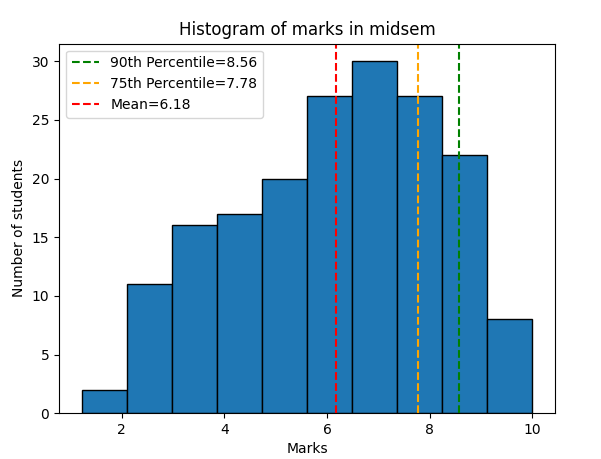
\includegraphics[width=\linewidth, height=5cm]{histogram.png} 
    \caption{Histogram for midsem marks}
    \end{subfigure}
    \begin{subfigure}{0.5\textwidth}
    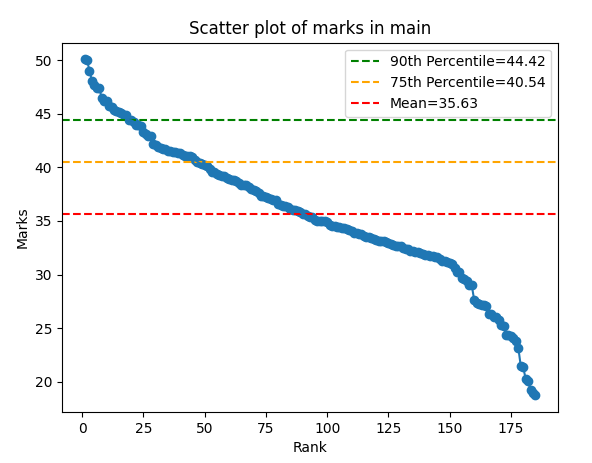
\includegraphics[width=\linewidth, height=5cm]{scatter-plot.png}
    \caption{Scatter plot for main.csv}
    \end{subfigure}
\end{figure}
\newpage

\subsection{Stats}
This command calls the \verb"stats.py" python script, which has a interface where users can choose between a particular exam or \verb"main" (for \verb"main", it considers the total marks for mark generation). It then displays the stats for that particular exam or \verb"main", if the csv file for the exam exists.\\
The stats include the mean, median, mode, standard deviation, $25^{th}$ percentile, $75^{th}$ percentile, $90^{th}$ percentile and maximum marks.\\
All these stats are calculated by calling their respective functions from \verb"stats_functions.py".\\

\textbf{Modules used for stats generation: os, csv, statistics}\\

\textbf{Script files: stats.py, stats\_functions.py}\\
\begin{center}
    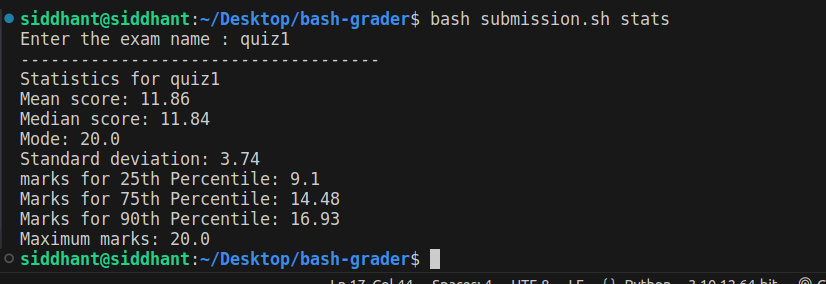
\includegraphics[height=5cm,width=10cm]{stats.png}
\end{center}

\subsection{Report Card}
This command calls the \verb"report_card.py" python script, which has a interface where users can choose between a particular student or all students. It then displays the report card for that particular student or saves the pdf of all student report cards in the \verb"report_cards" folder in the current directory.\\

It gets the grades and percentile rubrics for the grades from the instructor by calling functions from the \verb"grade.py" script. It then gets all the exams conducted and the maximum marks scored in each of these exams. Student marks for all students are also fetched by using the module \verb"csv".\\ It then calculates the weighted percentage of each student by using the formula:
\begin{equation}
    W.P. = \frac{\sum_{i=1}^{n} {M_i} \times {M_{max_i}}}{\sum_{i=1}^{n} {M_{max_i}}^2} \times 100\\
\end{equation}
where $M_i$ is the marks scored by the student in exam i, $M_{max_i}$ is the maximum marks scored in exam i and $n$ is the number of exams.\\

This is considering the maximum marks scored in each exam as the total marks for that exam. This ensures that a person with more marks in an exam with a greater weightage gets a higher weighted percentage.\\

The script then calculates the grade of each student by using the weighted percentage and the rubrics provided by the instructor. Then the percentiles of each student are calcualted with this weighted percentage using the \verb"scipy" module.
Then, the report card is generated from a template report card and text is put on the template using the \verb"PIL" module and then converted to pdf form for all students, while it's only displayed for one person.

\begin{center}
    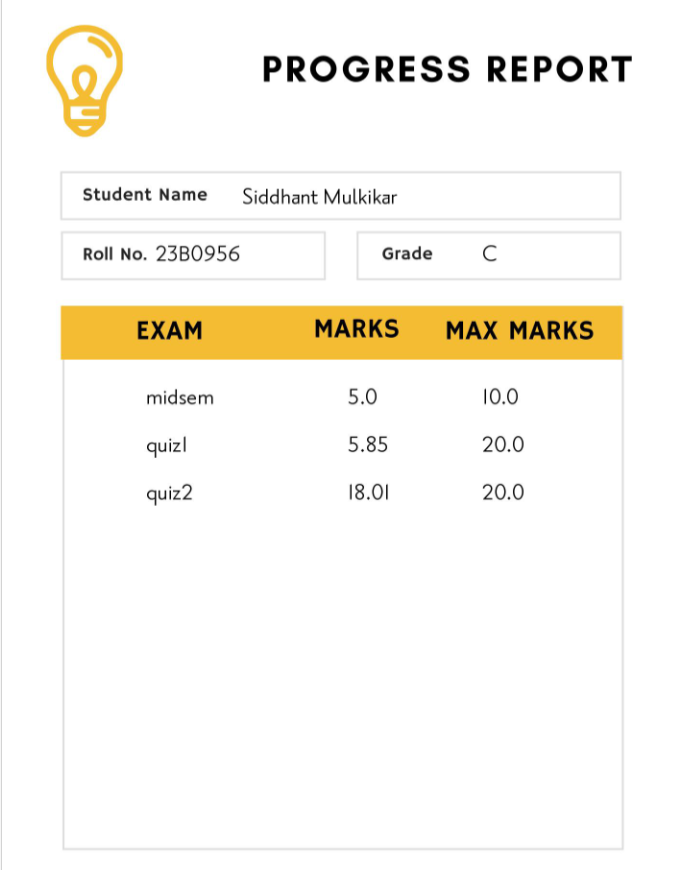
\includegraphics[height=10cm,width=8cm]{report-card.png}
\end{center}

\textbf{Modules used for report card generation: os, csv, statistics, scipy, PIL}\\

\textbf{Script files: report\_card.py, grade.py}

\begin{thebiblography}{9}

\bibliographystyle{plain}

\bibitem{bash}Bash \url{https://www.gnu.org/software/bash/manual/bash.html}
\bibitem{awk} \url{https://www.gnu.org/software/gawk/manual/gawk.html}
\bibitem{python} \url{https://docs.python.org/3/}
\bibitem{matplotlib} \url{https://matplotlib.org/}
\bibitem{scipy} \url{https://www.scipy.org/}
\bibitem{PIL} \url{https://pillow.readthedocs.io/en/stable/}
    \bibitem{csv} \url{https://docs.python.org/3/library/csv.html

\bibitem{os} \url{https://docs.python.org/3/library/os.html}
\end{thebibliography}

\end{document}

